\section{A finite alphabet with deterministic recovery}
\label{sec:labeling}

We construct a labeled graph in layers, with the aim that every sufficiently
long immersed word has only one occurrence.  The alphabet must also remain
small relative to the incidence degrees.  The finite-alphabet separation
objective is shared with Osajda's construction
\cite[\S\S2.1--2.3, Theorem~2.7]{Osa20}; here the graph and its labels are
built together, and uniqueness will follow from explicit recovery of vertex
coordinates.

The local recovery step is elementary.  Over a finite field, subtracting
two evaluations $E_1=v+c_1u$ and $E_2=v+c_2u$ with $c_1\ne c_2$
determines $u$; either equation then determines $v$.  We apply this
observation block by block.  Labels and previously recovered neighboring
blocks will supply the evaluations.  The rules below make this process
compatible with partial terminal blocks and with comparisons between
different heights.

A \emph{slot} is a named candidate incidence at a vertex.  Once the
coefficient pools are fixed, the incidence, recovery, and vertex-deletion
assertions in this section hold for every choice of permutation tables.
Deletion fractions are counted using uniform vertex coordinates for each
fixed table realization.  The probability law on the tables is a separate
choice, made in Section~\ref{sec:expansion}.  All logarithms in this section
have base two.

The padded-stream construction and recovery scheme adapt
\cite[Sections~4 and~6]{OpenAIProjection}.  The exponents, cutoff requirements,
and gated corrections needed for the present interfaces are established
below; the projection theorem is not an existence input.

\subsection{States, families, and extra coordinates}

Fix a positive integer $b$.  Let $s$ be a sufficiently large multiple of
$20000$ and $5b$, and put
\begin{equation}\label{eq:label-parameters}
 r=\frac35s,\qquad d=2^{.40005s},\qquad
 D=2^{.60005s},\qquad q=2^{.50005s}.
\end{equation}
The numbers $d,D$ will be the two incidence degrees in a fixed slice,
and $q=\sqrt{dD}$ their geometric mean.  The exponent choices allow both
distinct coefficients for recovery and an alphabet whose square root is
small compared with $q$; the precise alphabet estimate is
\eqref{eq:sharp-alphabet} below.
These parameters stay fixed as the height $i$ varies.  They may change
when a later construction asks for a smaller approximation error.
Choose an integer $n_0\ge 10^6$, to be increased later.  For $i\ge0$ write
$bi=2s a_i+t_i$, where $0\le t_i<2s$, and define
\begin{align}
 \ell_A(i)&=r+n_0s+a_is+\max\{t_i-s,0\},\notag\\
 \ell_B(i)&=n_0s+a_is+\min\{t_i,s\},\label{eq:stream-lengths}\\
 \mathscr A_i&=\F_2^{\ell_A(i)}\times\F_2^{r+\ell_B(i)},\qquad
 \mathscr B_i=\F_2^{\ell_B(i)}\times\F_2^{s-r+\ell_A(i)}.\notag
\end{align}
The two coordinates are denoted $(u,v)$.  Regard each as an infinite bit
stream by adjoining zero coordinates.  Both coordinates on a side use
that side's block convention: an A stream has an initial block
$A_0$ of length $r$ and blocks $A_1,A_2,\ldots$ of length $s$; a B stream
has blocks $B_1,B_2,\ldots$, all of length $s$.  Index their interleaving by
\begin{equation}\label{eq:source-order}
 A_0\ (0),\ B_1\ (1),\ A_1\ (2),\ B_2\ (3),\ A_2\ (4),\ldots.
\end{equation}
For the pair of spaces at height $i$, the active coordinates of $u_A$ and
$u_B$ together form an initial segment of this interleaving.  Its length
and the logarithmic state size are
\begin{equation}\label{eq:state-sizes}
 \begin{aligned}
 L_i&=r+2n_0s+bi,&
 H_i&=L_i+s-r=(2n_0+1)s+bi,\\
 |\mathscr B_i|&=2^{H_i},&
 |\mathscr A_i|&=2^{H_i+2r-s}.
 \end{aligned}
\end{equation}
Set $m_i=H_i/\log q$.  We require, by increasing $s$,
\begin{equation}\label{eq:label-slope}
 a:=\frac b{\log q}\le10^{-6}.
\end{equation}

Let $\mathcal T$ be any fixed finite set of incidence types.  A type
$\tau$ specifies an offset $\delta_\tau\in\{-1,0,1\}$ and occurs between
$\mathscr A_i$ and $\mathscr B_{i+\delta_\tau}$ whenever both indices are
nonnegative.  Put $T=|\mathcal T|$ and
\begin{equation}\label{eq:family-modulus}
 M=2\cdot10^6s.
\end{equation}
The family of this pair is $f=(\tau,i\bmod M)$.  Thus there are at most
$TM$ families.  Its two endpoint residues, its smaller height
$h=\min\{i,i+\delta_\tau\}$ modulo $M$, and the phase of its cutoff are
determined by $f$.

For an adjacent pair, truncate the larger endpoint to the coordinate
lengths at height $h$.  Exactly $b$ coordinates are discarded: they belong
to its $u$ coordinate if that side's $u$ stream grows from $h$ to $h+1$,
and otherwise to its $v$ coordinate.  They form one interval of $b$ bits,
since $s,r$ and every active length are multiples of $b$.  Denote their
value by $e\in\F_2^b$.  For an equal-height pair let $e$ be the empty
string.  In a fixed $e$ slice, both truncated endpoint spaces are exactly
the spaces at height $h$ in \eqref{eq:stream-lengths}.

At an A endpoint a slot has serial number $j\in\{1,\ldots,d\}$; at a B
endpoint it has, in addition, a bucket $c\in\F_2^{2r-s}$.  The type is
always part of a slot name.  At the smaller endpoint of an adjacent pair,
$e$ is also part of its slot name.  At the larger endpoint it is read from
the state.  Every positive incidence is oriented from its $\mathscr A$ endpoint to
its $\mathscr B$ endpoint. A positive edge label will be
\begin{equation}\label{eq:positive-label}
 \lambda=(f,j,e,h_0),\qquad h_0=c\Vert h_0',\quad
 |h_0|=r,\quad |h_0'|=s-r.
\end{equation}
Negative labels are formal inverses.  The notation $h_0$ here is a label
head, not a height.

For each family, mark its common $u$ cutoff $L_h$ at every actual
occurrence.  Let $\kappa$ be the source-block index of the last active
common $u$ block and $t\in\{b,2b,\ldots,s\}$ its active prefix length.
Also mark the interval of extra coordinates at each adjacent occurrence.
For consecutive occurrences of one family both side lengths increase by
$Mb/2$, and the indices $\kappa$ increase by
\begin{equation}\label{eq:mark-spacing}
 K=Mb/s=2\cdot10^6b.
\end{equation}
The marked prefix length and its side therefore remain the same within
a family.  The raw $u$ data of its actual endpoint pair extend at most
one source block beyond its common cutoff.  An extra $v$ interval lies
at most two source blocks beyond that cutoff, when its coordinate blocks
are indexed by \eqref{eq:source-order}.

\subsection{Finite coefficient pools}

An A coefficient name is $(f,j,e)$, and a B coefficient name is
$(f,j,c,e)$.  We include every legal value, including values of $e$ read
from the larger state.  In particular an A name does not contain the
bucket, which has not yet been read when its label head is computed.
Let $\mathcal N_A,\mathcal N_B$ be these two finite sets.  Their sizes
satisfy
\begin{equation}\label{eq:name-count}
 |\mathcal N_A|\le TM2^b d,\qquad
 |\mathcal N_B|\le TM2^bD.
\end{equation}
Choose an injection of $\mathcal N_A$ into $\F_{2^r}$ and an injection of
$\mathcal N_A\sqcup\mathcal N_B$ into $\F_{2^s}$.  Identify these fields
linearly with their bit-coordinate spaces.  The first injection acts on
block $A_0$; the second acts on every full $s$-block.  For a name $\nu$,
write $K_\nu$ for the block-diagonal map that multiplies each block by
its assigned field element, expressed in bit coordinates.
The same coefficients are used on every repeated block.
The finite fields used here introduce no group elements: for each $h$,
the roots of $z^{2^h}-z$ in a splitting field over $\F_2$ form a field
of $2^h$ elements, since the polynomial has derivative $-1$ and its
roots are closed under the field operations.

Distinct coefficients make the two-evaluation recovery step possible.
Expansion requires a second property: after restricting to an active
prefix, no output functional should give the same input functional on
too many slots.  The next lemma supplies this multiplicity bound as well
as distinctness; Section~\ref{sec:expansion} uses it to estimate the mean
incidence operator.

\begin{lemma}[Coefficient choice]\label{lem:coefficient-pools}
For sufficiently large $s$, the injections can be chosen so that, within
every fixed family and extra slice and on either side, the following
holds.  If $n$ is its number of slots, $\zeta$ is any nonzero output
linear functional on an ordinary $s$-block, and $b\le t\le s$, then each
restricted input functional
\[
  (\zeta K_\nu)|_{\F_2^t}
\]
occurs on at most $2^{1-b}n$ slots.  All distinct names have distinct
coefficients in every field in which they occur.
The analogous bound holds on the initial A field for every prefix
length between $b$ and $r$.
\end{lemma}

\begin{proof}
The injections exist because the polynomial factor $TM$ and fixed factor
$2^b$ in \eqref{eq:name-count} are dominated by the positive exponent
gaps $r-.40005s$ and $s-.60005s$.  Choose both injections uniformly.
For fixed nonzero $\zeta$, multiplication identifies the field
coefficients bijectively with all output-to-input functionals.  On any
specified set of $n$ names these are therefore sampled without
replacement.  Restriction to $t$ input bits has fibers of proportion
$2^{-t}\le2^{-b}$.

Here is the required tail estimate.  For $n$ zero--one samples without
replacement, with sum $S$ and mean success proportion $p$, one has
\[
 \mathbb E\exp(u(S-np))\le\exp(nu^2/8).
\]
Indeed the exponential moment before centering is an elementary
symmetric mean in the population entries $1,e^u$.  Replacing two unequal
nonnegative entries by their average increases every elementary
symmetric sum: the only changing term is their product multiplied by
a nonnegative symmetric sum in the other entries.  Iteration compares
the moment with sampling with replacement.  For a centered Bernoulli
variable, the second derivative of the logarithmic moment generating
function is a tilted variance, at most $1/4$; integrating twice proves
the displayed bound.  Exponential Markov inequality gives
\[
 \Pr\{S-np\ge 2^{-b}n\}\le
 \exp(-2^{1-2b}n).
\]
There are at most $s2^{2s}$ choices of an output functional, prefix length,
and restricted value.  Multiplying by the polynomial number of families
and the fixed number of extra slices and sides still gives $2^{O(s)}$
tests.  Each has $n\ge d=2^{.40005s}$.  Their total failure probability
tends to zero.  Fix a choice for which none fails.
\end{proof}

\subsection{Universal corrections and permutation rules}

The edge equations will couple each affine evaluation to a permuted
input block at the opposite endpoint.  To compare occurrences at different
heights, we use one system of equations on arbitrary padded streams.
The corrections remove the extra coordinates of an adjacent-height pair,
while the gates and identity blocks preserve the padded tail.  Their
dependence on earlier raw inputs is what will let recovery proceed one
block at a time.

We now specify these rules on arbitrary padded raw $u_A,u_B$ streams,
not only on actual endpoint states.  A pair of full raw blocks means
$(B_j,A_j)$ for $j\ge1$.  For a source-block index $k>20$, put
$J(k)=\lfloor(k-5)/2\rfloor$ and let
\begin{equation}\label{eq:lag-gate}
 g_k=1\quad\Longleftrightarrow\quad
 (u_{B,J(k)-3},u_{A,J(k)-3},\ldots,
   u_{B,J(k)},u_{A,J(k)})\ne0.
\end{equation}
For $k\le20$ put $g_k=1$.  Thus every noninitial gate reads exactly
eight full raw blocks and reads no source-block index greater than
$k-5$.  In particular a correction to an evaluation block cannot
consult the source block that will be recovered from that evaluation.

Fix a positive label \eqref{eq:positive-label}.  At every marked extra
interval of its family, XOR $e$ into that raw coordinate interval if
$g_k=1$, where $k$ is the coordinate-block index containing the interval.
There are no corrections for an equal-height family.  Denote the resulting
streams by
\begin{equation}\label{eq:corrected-streams}
 \bar u_C=u_C+C^u_{C,\lambda},\qquad
 \bar v_C=v_C+C^v_{C,\lambda},\qquad C\in\{A,B\}.
\end{equation}
The sums are XOR sums; each finite prefix uses finitely many disjoint
marked intervals.  Every correction offset in a block is determined by
the label and raw $u$ blocks strictly before both blocks coupled by the
edge equation below.  This extra lag is deliberate.

For every family, label, source-block index $k$, and tuple of all raw $u$
blocks strictly earlier than $k$ in \eqref{eq:source-order}, provide a
permutation table.  At an unmarked index it is a permutation of the full
block; at a marked cutoff with active length $t$ it is a permutation of
$\F_2^t$.  These are distinct variables for distinct complete keys.  There
are finitely many variables at each source-block index.

The transformation at a source block is defined as follows.
\begin{enumerate}
\item At each marked cutoff use its prefix table on the first $t$ bits
and the identity on the suffix, if $g_k=1$; if $g_k=0$, use the identity
on the entire block.
\item At the twenty source blocks immediately following every marked
cutoff, use the identity unconditionally.
\item At every other source block use its full-block table if $g_k=1$,
and otherwise the identity.
\end{enumerate}
The marked and following intervals do not overlap by
\eqref{eq:mark-spacing}.  Tables act on corrected $\bar u$ blocks, while
their keys and gates read raw preceding $u$ blocks.  Write
$P_{A,\lambda}(\bar u_A)$ and $P_{B,\lambda}(\bar u_B)$ for the two
transformed streams.  For a fixed slot write
$Q_C=\bar v_C+K_\nu\bar u_C$ for its corrected evaluation; the slot
and label subscripts will usually be suppressed.  Its difference from
the raw evaluation $v_C+K_\nu u_C$ is the known correction offset
$C^v_{C,\lambda}+K_\nu C^u_{C,\lambda}$.
The universal edge equations are
\begin{equation}\label{eq:universal-edge-equations}
 \boxed{\quad
 \bar v_A+K_{(f,j,e)}\bar u_A
       =h_0\Vert P_{B,\lambda}(\bar u_B),\qquad
 \bar v_B+K_{(f,j,c,e)}\bar u_B
       =h_0'\Vert P_{A,\lambda}(\bar u_A).
 \quad}
\end{equation}
They are equations of infinite padded streams.

For the auxiliary incidence at an actual pair, modify these rules at
that occurrence only: force its extra correction on, if there is one,
and force its current final-prefix permutation on.  All lower rules
retain their gates.  Denote this auxiliary prescription by a superscript
$0$.  We shall delete states for which either forced choice was necessary.
The sparse unconditional identity zones replace any need for a
post-cutoff gate that could inadvertently read the raw extra bits.

\subsection{Auxiliary incidences and uniform coordinates}

The auxiliary prescription gives a finite incidence at every height pair.
We first verify that its equations preserve the required supports, then
solve them in either direction.  The same inversion will identify the
uniform coordinates used to count gate failures.

\begin{lemma}[Inversion and uniform coordinates]\label{lem:incidence-inversion}
For every choice of tables the auxiliary prescription has exactly one
edge at every specified endpoint and slot.  In a fixed extra slice it is
biregular of degrees $d,D$.  A uniform endpoint with a fixed slot, after
fixing its extra value when necessary, is parametrized bijectively by
the free label head and all free raw $u_A,u_B$ coordinates at the common
cutoff.  Consequently those raw coordinates are independent uniform bits.
\end{lemma}

\begin{proof}
\emph{Preservation of the common support.}
At the actual larger endpoint the forced correction cancels its extra
bits.  Lower correction intervals lie in active coordinates.  Higher
correction gates vanish: their eight preceding raw blocks are wholly
beyond the actual endpoint support, because consecutive marks are
separated by $K>20$ source blocks.  Thus corrected streams have exactly
the common permitted lengths.

The transformed corrected $u$ streams preserve these lengths.  At the
last common block the suffix is the identity.  The next twenty blocks
are identity, and their corrected inputs are zero.  Raw $u$ support
extends by at most one block beyond the common cutoff.  At every later
ordinary index the gate window \eqref{eq:lag-gate} is entirely beyond
that support, so its gate is closed.  The same holds at all higher
marked rules.  This proves preservation of the padded tail, including
an extra interval in the larger endpoint's $u$ coordinate.

For clarity, the two possible common terminal shapes are
\begin{equation}\label{eq:terminal-shapes}
\begin{array}{c|cccc}
 &\ell_A&\ell_B&|v_A|&|v_B|\\ \hline
 \text{last B prefix }t&r+ns&ns+t&r+ns+t&(n+1)s\\
 \text{last A prefix }t&r+ns+t&(n+1)s&r+(n+1)s&(n+1)s+t .
\end{array}
\end{equation}
In both rows $1\le t\le s$ and the output of each block-diagonal $K$
fits in the displayed $v$ length.  If an extra interval is in $v$, it
lies beyond this output: its same-side direct block is zero there.
Thus computing $v$ from the equations cannot leak a $K u$ term into
the prescribed extra interval.

\emph{Inversion from either endpoint.}
Given an A endpoint and slot, its extra value is known, either from the
state or from the slot.  Its first $r$ evaluation bits determine $h_0$;
there are no marked corrections in the initial blocks.  Hence $c$ and
the B coefficient name are known.  Proceed through the B blocks.  To
compute its next corrected evaluation from the A endpoint, all correction
gates use already known raw blocks by their five-index lag.  The B
permutation key uses only earlier B blocks and the preceding A block.
Invert that known block permutation, then undo the known correction to
recover the next raw B $u$ block.  The other equation now determines its
raw $v$ block.  Continue in order.  The support argument just given shows
that all recovered streams have the required lengths.

Conversely a B slot gives $c$.  Its first $s-r$ evaluation bits give
$h_0'$, and hence $h_0$.  Inverting successive A block permutations
recovers raw $u_A$ and then $v_A$.  These two procedures solve the same
triangular equations and are inverse.  The lag is important here: a
correction in $Q_{B,j}$ does not read the unknown $u_{A,j-1}$, and one
in $Q_{A,j}$ does not read the unknown $u_{B,j}$.

\emph{Uniform coordinates.}
First freely specify the raw $u$ blocks on
both sides, omitting only the larger endpoint's fixed extra interval if
that interval is in $u$.  Specify $h_0$ for an A slot, or $h_0'$ for a B
slot whose bucket is fixed.  Every gate, correction, and permutation
value is now determined.  Equations \eqref{eq:universal-edge-equations}
determine both $\bar v$ streams, and undoing the corrections determines
both raw $v$ streams.  A forced extra interval in $v$ is exactly $e$.
The number of free coordinates is
\[
 \ell_A(h)+\ell_B(h)+r=\log|\mathscr A_h|
 \quad\hbox{or}\quad
 \ell_A(h)+\ell_B(h)+s-r=\log|\mathscr B_h|,
\]
respectively.  The preceding inversion proves bijectivity, not merely
equality of dimensions.  Uniform measure therefore becomes product
uniform measure in these coordinates.
\end{proof}

\subsection{Deleting gate failures}

Let $X^0$ be the union of the auxiliary incidences over all types and
height pairs.  At a slot, evaluate the natural gates on its auxiliary
edge, even where the auxiliary prescription forced them on.  If its
common last source-block index is $\kappa$, delete an endpoint state if
any of the following holds for any incident slot:
\begin{enumerate}
\item One of $g_{\kappa},g_{\kappa-1},g_{\kappa-2}$ is zero.
\item The natural gate at its actual extra correction interval is zero.
This test is omitted for equal-height pairs.
\item Among the full active A source blocks other than $A_0$, more than
$1/250$ of their gates are closed; or the same holds among the full
active B source blocks.  These are separate tests for the two parities.
\end{enumerate}
The last test counts ordinary gate closures; deterministic marked and
following identity blocks will be accounted for separately.

\begin{lemma}[Uniform gate budget]\label{lem:gate-deletions}
For every fixed set of tables, the fraction deleted for gate reasons
from either state space at any height is at most
\begin{equation}\label{eq:gate-budget}
 \varepsilon_{\rm gate}=600T2^bD\,2^{-8s}.
\end{equation}
On a surviving edge both auxiliary forced choices were unnecessary, so
the edge satisfies the universal padded equations
\eqref{eq:universal-edge-equations}.  At each surviving slot, separately
among its full A source blocks and its full B source blocks, fewer than
$.005$ of the updates are unavailable because of a closed gate or a
marked or following deterministic identity rule.  The last three source
gates and the actual prefix gate are open.
\end{lemma}

\begin{proof}
Fix a slot and, where necessary, condition on its actual extra value.
Every gate tested at or before the common cutoff, and the gate of the
extra interval at most two blocks later, reads eight full free raw
$u$ blocks.  They are independent uniform by
Lemma~\ref{lem:incidence-inversion}.  Thus each noninitial gate is closed
with probability exactly $2^{-8s}$.  Initial gates are never closed.
Each parity in the third test has at least $n_0$ full active blocks.
Linearity of expectation and Markov's inequality give probability at
most $250\,2^{-8s}$ for each of its two failures.  The first two tests
add at most $4\,2^{-8s}$.  There are at most $T2^bD$ slots at either
endpoint, since $D\ge d$.  A union bound proves
\eqref{eq:gate-budget}, with room in the constant.  Averaging over the
extra value gives the same bound at a larger endpoint.

The first two tests refer only to raw coordinates obtained before the
forced choices can matter.  If they pass, the auxiliary and universal
rules coincide along this edge; the padding argument of
Lemma~\ref{lem:incidence-inversion} applies to both ends.  Restricting to
edges with two surviving endpoints therefore gives a subgraph satisfying
the universal equations.

For either source parity, the fraction of full active blocks belonging
to marked or following twenty-block zones is at most
\[
 \frac{22}{K}+\frac{22}{n_0}<10^{-4}.
\]
Indeed these zones have at most eleven indices of each parity, are
separated by $K$ interleaved indices, and there is at most one boundary
zone in the count.  The displayed larger constants cover both endpoints
of the counting interval.  Together with the separate $1/250$ gate
bound this is less than $.005$.  A marked partial block is counted as
unavailable for a full-$s$-bit test even if its prefix gate is open.
The current cutoff and its preceding two indices are not in a previous
marked zone, by \eqref{eq:mark-spacing}.
\end{proof}

\subsection{Recovery of arbitrary padded prefixes}

The gate deletion has made every surviving edge satisfy the same
universal equations.  We can now compare two occurrences of one label
word, even when their vertex states have different active lengths.
The distance of a position from the word's ends determines how much
of its padded state can be recovered.

For an A position put
\begin{equation}\label{eq:aligned-depths}
 \delta_A(j)=(2j+1)s\quad(j\ge0),\qquad
 \delta_B(j)=2js\quad(j\ge0).
\end{equation}
Depth $\delta_A(j)$ means both raw A streams through $r+js$ bits;
depth $\delta_B(j)$ means both raw B streams through $js$ bits.
In particular B depth zero contains no data.  The available common full
depth of a state, using only blocks in which both streams are active,
belongs to $[H_i-2s,H_i]$.  These conventions have the useful exact
identities
\begin{equation}\label{eq:depth-propagation}
 \delta_A(j)-\delta_B(j)=s\quad(j\ge0),
 \qquad \delta_B(j)-\delta_A(j-1)=s\quad(j\ge1).
\end{equation}
No $r$-dependent rounding error occurs when a coherent junction is
trimmed by one edge at each end.

The radius of a position on a path is its smaller distance in edges to
the two endpoints.  A path is immersed if it does not immediately
traverse an edge and then its reverse.

\begin{lemma}[Padded-prefix recovery]\label{lem:tower-recovery}
Let two immersed paths in the gate-surviving graph have the same
oriented label word.  At corresponding A positions of radius at least
$2j+1$, both raw streams agree through $r+js$ bits.  At corresponding B
positions of radius at least $2j$, both raw streams agree through $js$
bits.  These statements compare padded coordinates, so the positions
may have arbitrarily different heights.
\end{lemma}

\begin{proof}
The label orientation identifies the side, and the complete label
identifies the family, both coefficient names, the extras, and every
universal rule.  At an interior vertex the two incident coefficient
names are distinct.  Otherwise, at A their family, serial and actual
extra agree, and at B their bucket agrees as well; they are the same
slot.  The unique-edge assertion in Lemma~\ref{lem:incidence-inversion}
would then make the path backtrack.

For either incident name $\nu$, rearrange its current corrected
evaluation block as
\begin{equation}\label{eq:recovery-linear-equation}
 v+K_\nu u=R_\nu+C^v_\nu+K_\nu C^u_\nu.
\end{equation}
If the right sides and correction offsets are known for the two names,
their difference recovers the entire raw $u$ block because the difference
of the field coefficients is nonzero.  Then either equation recovers
the raw $v$ block.  The argument applies to full padded blocks even
when an actual endpoint has only a partial active block.

At an A position of radius one, the two first evaluations are precisely
the two label heads, and the initial correction offsets vanish.  This
recovers $A_0$.  Suppose next that $j\ge1$.  At a B position of radius
$2j$, each neighbor has A radius at least $2j-1$, so its raw streams are
known through block $A_{j-1}$ by induction.  The central B streams are
already known through $B_{j-1}$.  To compute the required right side of
the second equation in \eqref{eq:universal-edge-equations} through $js$
bits, one needs only the A transformed stream through
\[
 js-(s-r)=r+s(j-1).
\]
Every key for its last needed source block uses A blocks strictly before
$A_{j-1}$ and central B blocks through $B_{j-1}$.  Its argument is the
already recovered full corrected $A_{j-1}$ block.  Its gates and all
correction offsets use still earlier raw blocks by
\eqref{eq:lag-gate}.  Thus the two right sides are known, and
\eqref{eq:recovery-linear-equation} recovers $B_j$.

At an A position of radius $2j+1$, both neighbors have B radius $2j$.
The first edge equation through $r+js$ uses the B transformed stream
through $js$.  Its last argument is the already recovered corrected
$B_j$ block, and its keys use central A blocks only through $A_{j-1}$
and earlier B blocks.  Again the correction lag makes every offset
known.  Subtraction recovers $A_j$.

This induction is an induction on individual source blocks, not on
whole A--B pairs.  At each step both table keys and table arguments
are known before any current output is used.  The universal rules
are identical in the two occurrences, including at marked cutoffs
lying beyond one actual state's support.  Padding therefore causes
no exception to the induction.
\end{proof}

Figure~\ref{fig:stream-causality} summarizes this induction.
\begin{figure}[tbp]
  \centering
  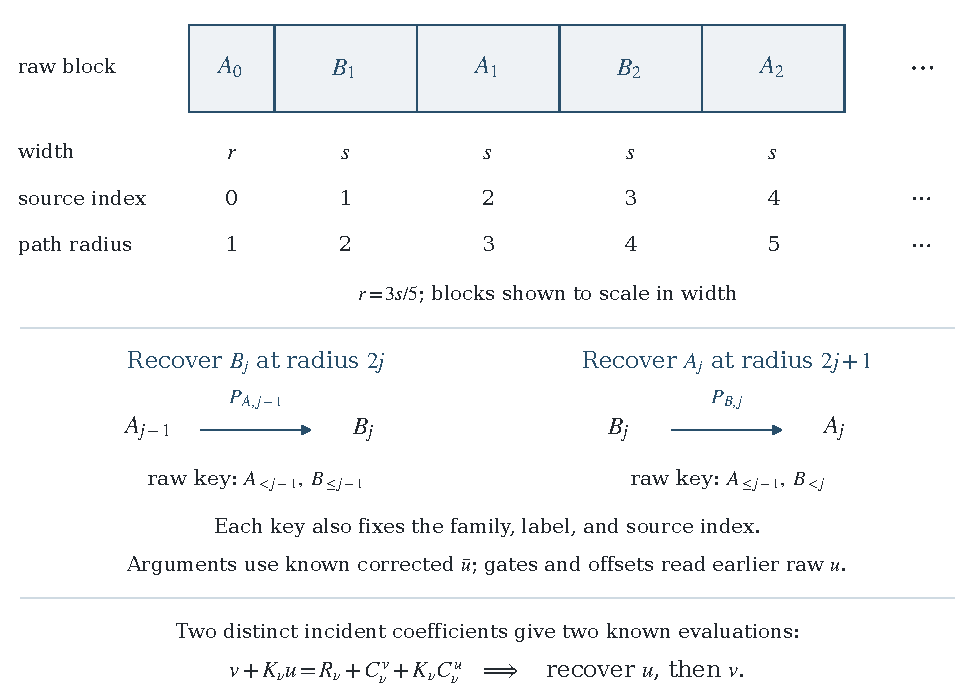
\includegraphics[width=\linewidth]{figures/stream-causality.pdf}
  \caption{Interleaving and the recovery induction of
  Lemma~\ref{lem:tower-recovery}. The radius shown suffices to recover both
  raw streams through that side's indicated block. Each arrow supplies an
  evaluation from a recovered neighbor block; two incident coefficients
  recover the receiver's $u,v$. Key abbreviations denote raw $u$ blocks.
  At the first B step, $h'_0$ supplies the initial $s-r$ evaluation bits.
  Tables act on corrected arguments; keys and gates read earlier raw
  inputs, with the lag in \eqref{eq:lag-gate}.}
  \label{fig:stream-causality}
\end{figure}

\subsection{Separating all heights}

Recovery will determine the complete state at a midpoint once a word is
long enough.  It does not yet identify the height: a shorter state might
agree with the padded prefix of a longer one.  The following deletion
excludes precisely the zero extensions needed for that ambiguity.

Put $\eta_{\rm sep}=1/2500=.0004$.  For a vertex on side $C$ at height $i$, and
each $i'<i$ with $i'\equiv i\pmod M$, let
\begin{equation}\label{eq:separation-interval}
 \Delta=\ell_C(i)-\ell_C(i')=(i-i')b/2,\qquad
 q(i,i')=\left\lfloor\min\{\eta_{\rm sep} H_{i'},\Delta\}\right\rfloor.
\end{equation}
Delete the vertex if its $q(i,i')$ raw $u_C$ bits immediately following
the smaller cutoff $\ell_C(i')$ are all zero.  These are active bits
at height $i$.  Denote by $X^{\rm good}$ the graph induced from $X^0$
after the gate and separation deletions.

\begin{lemma}[Uniform separation budget]\label{lem:separation-deletions}
The fraction deleted for separation from either side at any height is
at most
\begin{equation}\label{eq:separation-budget}
 \varepsilon_{\rm sep}
 =2\left(
 \frac{2^{-Mb/2}}{1-2^{-Mb/2}}
 +\frac{2^{-\eta_{\rm sep} H_0}}{1-2^{-\eta_{\rm sep} b}}
 \right).
\end{equation}
\end{lemma}

\begin{proof}
Uniform raw vertex coordinates are independent bits.  The probability
of the test for $i'$ is $2^{-q(i,i')}$.  The elementary inequality
\[
 2^{-\lfloor\min(x,y)\rfloor}\le2(2^{-x}+2^{-y})
\]
splits its bound into a term depending on the smaller height and one
depending on the height difference.  Summing the latter over positive
multiples of $M$, and the former even over all nonnegative smaller
heights, gives \eqref{eq:separation-budget}.  Both sums converge
uniformly in the larger height.
\end{proof}

\begin{proposition}[The deterministic labeled tower]\label{prop:tower-labels}
For every fixed finite type set and every sufficiently large $s$ as
above, the construction has the following properties.
\begin{enumerate}
\item The auxiliary state sizes are \eqref{eq:state-sizes}.  In a fixed
extra slice an incidence has degrees $d,D$.  Without slicing, its
smaller side acquires the extra factor $2^b$ and its larger side does
not.  The total degrees are at most $T2^b d$ on A and $T2^bD$ on B.
\item The labeling is folded: no two outgoing oriented edges at a
vertex have the same label.  Its signed alphabet satisfies
\begin{equation}\label{eq:sharp-alphabet}
 |\mathcal S|\le 2TM2^b d2^r,
 \qquad
 \frac{\sqrt{|\mathcal S|}}q
 \le 2^{-.000025s+O(\log s)+O_{T,b}(1)}\longrightarrow0.
\end{equation}
\item At every height the fraction of removed vertices on each side is
at most $\varepsilon_{\rm gate}+\varepsilon_{\rm sep}$.  This bound can
be made arbitrarily small, uniformly over heights and all table choices.
The separate-parity and terminal gate conclusions of
Lemma~\ref{lem:gate-deletions} hold.
\item Every immersed path in $X^{\rm good}$ starting at height $i$ and
having length at least $\lceil1.002m_i\rceil$ is the unique immersed
path with that oriented word anywhere in $X^{\rm good}$.  This is a
global assertion over all heights and components.
\end{enumerate}
\end{proposition}

\begin{proof}
The degree statements follow from
Lemma~\ref{lem:incidence-inversion}.  At a larger endpoint, a fixed
state specifies its extra value; at a smaller endpoint that value
ranges over its slots.  At an A endpoint equal labels specify equal
serial, family, and extra, hence the same slot.  At B they also specify
the bucket.  Uniqueness of the edge at a slot proves foldedness, and
restriction to an induced subgraph preserves it.  Counting
\eqref{eq:positive-label} gives \eqref{eq:sharp-alphabet}; its exponent
uses $\log d+r=1.00005s$, not a coarser word-counting bound.
The deletion assertions are
Lemmas~\ref{lem:gate-deletions} and~\ref{lem:separation-deletions}.

For fixed $b$ and incidence types, the label count has logarithm at most
$1.00005s+O(\log s)$, whereas $\log_2(q^2)=1.0001s$.
This strict margin persists after fixed finite refinements of the labels.
It will make the weighted forest error tend to zero in
Lemma~\ref{lem:finite-profile-realization}.

It remains to prove global uniqueness.  Let
$N=\lceil1.002m_i\rceil$ and compare the first $N$ edges of two paths
with the same oriented word.  Their midpoint radius is at least
$\lfloor N/2\rfloor$.  If the first midpoint has height $j$, then
\[
 H_j\le H_i+bN\le(1+1.002a)H_i+b.
\]
By Lemma~\ref{lem:tower-recovery}, their common recovered aligned depth
$\delta$ satisfies
\[
 \delta\ge s(N/2-2)
 \ge\frac{1.002}{1.0001}H_i-2s
 \ge1.001H_j.
\]
The last inequality follows from $a\le10^{-6}$,
$H_i\ge(2\cdot10^6+1)s$, and $b/s=.50005a$.

For all heights, \eqref{eq:stream-lengths} gives
\begin{align*}
 \ell_A&\le H/2+.1s,& |v_A|&\le H/2+.6s,\\
 \ell_B&\le H/2,& |v_B|&\le H/2+.5s.
\end{align*}
An aligned A depth $\delta$ recovers $\delta/2+.1s$ bits of each
stream, and a B depth recovers $\delta/2$ bits.  Since $H_j\ge1000s$,
the displayed recovery covers the entire first midpoint state.

The labels give equal height residues at the two midpoint positions.
If their heights differ, write $i_-<i_+$ for them.  Their own-$u$
length difference is the $\Delta$ of
\eqref{eq:separation-interval}.  The smaller state's padding is zero
on the interval tested there at the larger state.  Its endpoint is at
most
\[
 (1/2+\eta_{\rm sep})H_{i_-}+.1s\quad\text{on A},\qquad
 (1/2+\eta_{\rm sep})H_{i_-}\quad\text{on B}.
\]
Because $H_{i_-}\le H_j$ and $2\eta_{\rm sep}<.001$, the recovered prefix
contains that whole interval, even if $i_+$ is arbitrarily large.
The larger state would therefore have failed its separation test,
a contradiction.  The two heights are equal.  Their entire states
agree by the recovery already proved.  Foldedness now identifies the
paths in both directions from this midpoint, and uniquely continues
any longer common word.
\end{proof}

\subsection{The interface with probabilistic selection}

\begin{remark}[Terminal dimensions]\label{rem:terminal-dimensions}
The two rows of \eqref{eq:terminal-shapes} give the exact terminal
dimension split needed later.  In the side containing a partial final
$u$ block, its final pair $(u,v)$ has dimensions $(t,s)$; the other side
has a final pair of dimensions $(0,t)$.  Two independent incident
evaluations impose respectively $s-t$ and $t$ compatibility bits.
The first assertion follows because multiplication by a nonzero
coefficient difference is injective on the active $t$-dimensional
subspace.  The second is simply equality of the two $t$-bit evaluations.
Thus the sum is exactly $s$.  For adjacent incidences first move each
known affine correction $C^v+K C^u$ intact to the other side of its
evaluation equation.  A change in one input bit can affect all output
coordinates under field multiplication; these known shifts cost no
random dimension.  Only the width of the common active random prefix
can cost compatibility bits.  Projection to such a prefix of width
$w'$ gives an image of dimension at most $w'+t$ in $2w'$ dimensions,
hence codimension at least $\max\{0,w'-t\}$.  The adjacent-cutoff and
block-boundary cases, including a newly deterministic fragment, are
proved in Lemma~\ref{lem:pruning-terminal-codimension}; they lose at
most $4b$ compatibility bits.  No injectivity of a truncated
coefficient difference is asserted.
The probabilistic use of these dimensions still requires distinct
current table variables; that issue is addressed in
Proposition~\ref{prop:pruning}.
\end{remark}

\begin{remark}[Inputs to the probabilistic stages]\label{rem:label-interface}
The uniform-coordinate statement is an assertion for each fixed table
realization.  Proposition~\ref{prop:sequential-law} may therefore choose
the tables successively while retaining all deletion budgets.  The current
tables are coordinatized in
Lemma~\ref{lem:fresh-matching-coordinates} below; they are independent
under the product reference law used there.  In reconstruction of a
fixed labeled candidate, endpoint free $u$ bits are enumeration data
fixed before sampling.  At update $B_j$ the queried argument of
$P_{A,j-1}$ is already known; at the following update $A_j$ the
argument of $P_{B,j}$ is already known.  Current untested outputs can
affect only later arguments.  Gates for XOR corrections use the
stronger lag \eqref{eq:lag-gate}; ordinary preceding-key dependence
alone would not suffice for those corrections.
\end{remark}
